\section{Ustalenia terminologiczne}
\begin{definicja}[Graf skierowany (DG)]\label{def:DG}
Powiedzmy, że:
\begin{enumerate}
\item \(V\neq\emptyset\) jest zbiorem
\item \( E \subseteq V \times V \)
\end{enumerate}
Grafem skierowanym \(G\) nazwiemy dwójkę \((V, E)\).
\end{definicja}

\begin{definicja}[Acykliczny graf skierowany (DAG)]\label{def:dag}
Acyklicznym grafem skierowanym nazywamy graf skierowany nie zawierający cykli.
\end{definicja}

\begin{definicja}[Domknięcie przechodnie grafu]\label{def:domk_przechodnie_grafu}
Niech \(G=(V,A)\) będzie grafem skierowanym. Graf skierowany \(G^+=(V,A^{+})\) nazywamy \textbf{domknięciem przechodnim} grafu \(G\), gdy \(A^{+}\) jest zbiorem wszystkich takich par \((a,b)\) wierzchołków zbioru \(V\), że w grafie \(G\) istnieje droga z \(a\) do \(b\).
\end{definicja}

\begin{definicja}[Zbiór przechodni]\label{def:transitive_set}
Zbiór \(A\) nazywamy \textbf{przechodnim}, wtedy i tylko wtedy, gdy
\(\forall{x}\left(x\in A \land y\in x\implies y\in A\right)\).  
\end{definicja}

\begin{definicja}[Domknięcie przechodnie zbioru]\label{def:transitive_closure_set}
Domknięciem przechodnim zbioru \(X\) nazywamy najmniejszy w sensie inkluzji zbiór przechodni, który zawiera \(X\).
\end{definicja}

\begin{definicja}[Graf zależności]\label{def:depend_graph}
Niech dane będą zbiór \(S\neq\emptyset\), relacja przechodnia \(R\subseteq S\times S\). \textbf{Grafem zależności} nazywamy graf \(G=(S,T)\) i \(T\subseteq R\), gdzie \(R\) jest przechodnim domknięciem \(T\).
\end{definicja}


\begin{definicja}[Ścieżka]\label{def:sciezka}
\textbf{Ścieżką} łączącą \(v_0\) z \(v_n\) o długości \(n\) nazywamy ciąg wierzchołków \((v_0, v_1, \dots, v_n)\) taki, że dla każdego \(k\in \{0, 1, \dots, n-1\}\) istnieje krawędź z \(v_k\) do \(v_{k+1}\).
\end{definicja}

\begin{definicja}[Droga]\label{def:droga}
\textbf{Drogą} w grafie \(G\) nazywamy ścieżkę, której wierzchołki są różne.
\end{definicja}

\begin{definicja}[Długość drogi]\label{def:dlugosc_drogi}
\textbf{Długością} drogi w grafie \(G\) nazywamy liczbę krawędzi, które zawiera droga.
\end{definicja}
\begin{definicja}[Cykl]\label{def:cykl_w_grafie}
Drogę zamkniętą długości co najmniej 1 z ciągiem wierzchołków \(x_1 x_2\dots x_n x_1\) nazywamy \textbf{cyklem}, jeśli wszystkie wierzchołki\\ \(x_1, x_2\dots x_n\) są różne.
\end{definicja}

\begin{definicja}[Stopień wierzchołka]\label{def:stopien_node}
\textbf{Stopień \(d_{G}(v)\) wierzchołka} \(v\) definiujemy jako liczbę incydentnych z \(v\) krawędzi. Każdemu wierzchołkowi \(v\) grafu skierowanego \(G\) możemy przypisać stopień wyjściowy (ang. \emph{indegree}) \(d_{G}^{+}(v)\) i stopień wejściowy (ang. \emph{outdegree}) \(d_{G}^{-}(v)\):
\begin{align*}
 d_{G}^{+}(v) = \#\{w|(v,w)\in E\}\\ 
 d_{G}^{-}(v) = \#\{w|(w,v)\in E\}
\end{align*}
\end{definicja}

\begin{definicja}[Macierz]\label{def:matrix}
Niech \(\mathbb{K}\) będzie ciałem. Macierzą o \(m\) wierszach i \(n\) kolumnach i wartościach w \(\mathbb{K}\) (krótko: macierzą \(m\times n\)) nazywamy każde odwzorowanie \(A:\{1,\dots, m\}\times \{1, \dots, n\}\xrightarrow{} \mathbb{K}, (i,j)\longmapsto A_{ij}\)
\end{definicja}

\newpage

\section{Klasyfikacja algorytmów}
\begin{definicja}[Algorytm]\label{def:algorytm}
Zbiór jednoznacznie określonych reguł lub zadań obliczeniowych prowadzących w skończonej ilości kroków do rozwiązania pewnego problemu \cite{IEEE}.
\end{definicja}


Określone w ten sposób zadania obliczeniowe są z reguły względem siebie niezależne. Pewne z zadań mogą być wykonywane równolegle, inne muszą być wykonywane sekwencyjnie, jedno po drugim. Wobec tego algorytm może być określony częściowo równolegle, częściowo sekwencyjnie.


Podstawowymi elemetami określającymi dowolny algorytm są:
\begin{enumerate}
\item zadania do wykoniania,
\item zależności pomiędzy zadaniami polegające na określeniu czy 
dane wyjściowe któregoś z zadań nie są danymi wejściowymi dla innego zadania,
\item zbiór danych wejściowych wymaganych przez algorytm,
\item zbiór danych wyjściowych otrzymywanych po wykonania algorytmu.
\end{enumerate}

%Na podstawie niezależności zadań obliczeniowych algorytmy możemy %podzielić na pięć klas \cite{APC2011}:
%\begin{enumerate}
%\item Algorytmy szeregowe
%\item Algorytmy równoległe
%\item Algorytmy szeregowo--równoległe (SPA, Serial--Parallel %Algorithms)
%\item Algorytmy nieszeregowo--równoległe (NSPA, Nonserial--%Parallel Algorithms)
%\item Algorytmy regularno-iteracyjne (RIA, Regular--Iterative %Algorithms)
%\end{enumerate}

\begin{definicja}[Algorytm sekwencyjny]\label{def:algorytm_sekwencyjny}
\textbf{Algorytm sekwencyjny} (rys.  \ref{fig:sequential}) jest ciągiem dokładnie sprecyzowanych zadań obliczeniowych \(T_i,\, i\in\mathbb{N}\) rozwiązujących dany problem, tj. wyznaczających dane wyjściowe na podstawie danych wejściowych. Zakłada się, że w algorytmie sekwencyjnym zadania wykonywane są przez jeden procesor.

\end{definicja}

\begin{figure}[h]
\centering
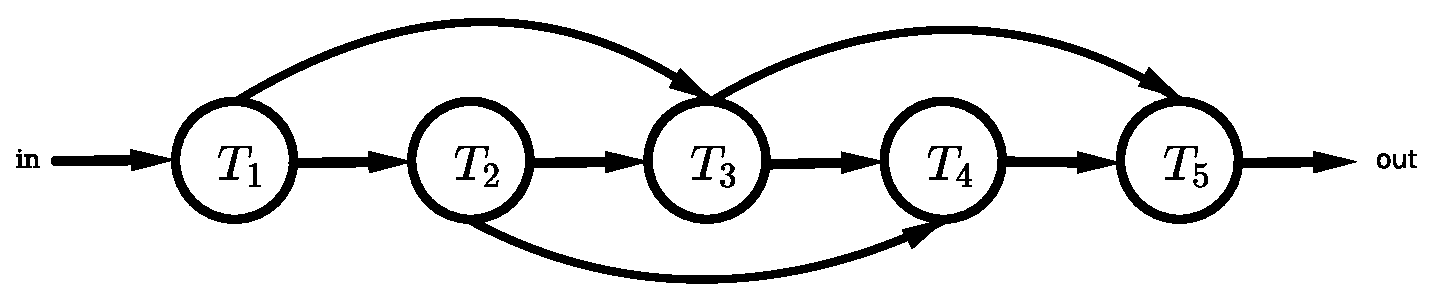
\includegraphics[width=14cm]{images/Rys2.eps}
\caption{Algorytm sekwencyjny}
\label{fig:sequential}
\end{figure}

W celu rozwiązania problemu za pomocą większej liczby procesorów należy go zdekomponować na podproblemy, które mogą być rozwiązane równolegle. Każdy z podproblemów rozwiązywany jest przez odrębny algorytm będący składową algorytmu równoległego.


\begin{definicja}[Równoległość]\label{def:rownoleglosc}
\textbf{Równoległość} w odniesieniu do oprogramowania jest to symultaniczny transfer, występowanie albo przetwarzanie poszczególnych części pewnej całości, takich jak bity składające się na znak albo znaki pewnego słowa, używając osobnych urządzeń dla ich różnych części \cite{IEEE}.
\end{definicja}


\begin{definicja}[Algorytm równoległy]\label{def:algorytm_rownolegly}
\textbf{Algorytmem równoległym} (rys. \ref{fig:parallel}) nazywamy każdy algorytm, w którym spośród określonych w nim zadań \(T_1\), \(T_2\), \(\dots\), \(T_n\) co najmniej dwa zadania \(T_i\), \(T_j\), \(i\neq j\) dzięki ich wzajemnej niezależności, mogą być wykonane równocześnie \cite{APC2011}.\\
\end{definicja}

\begin{figure}[h]
\centering
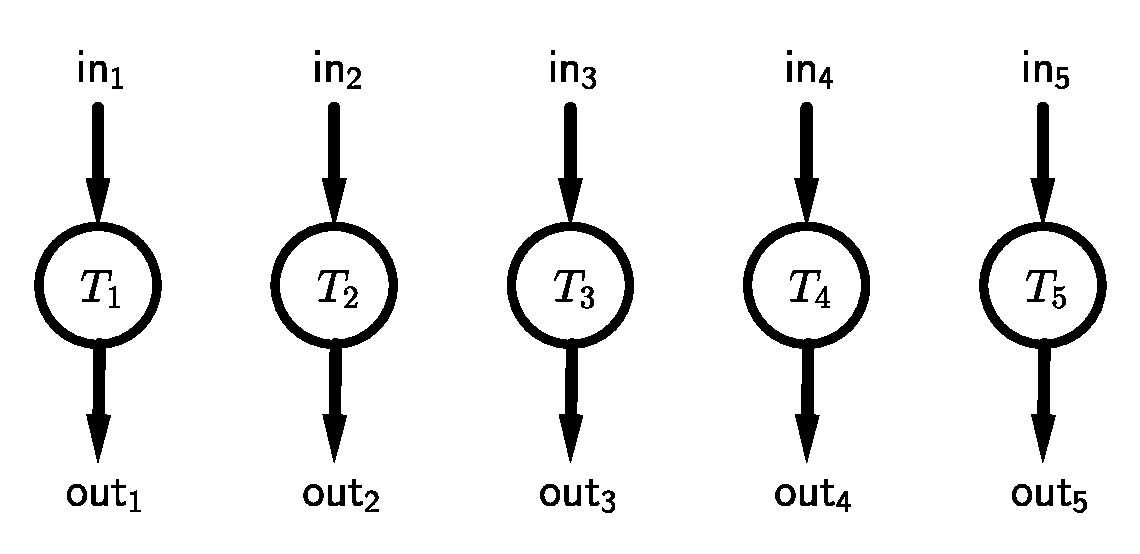
\includegraphics[width=10cm]{images/Rys1.eps}
\caption{Algorytm równoległy}
\label{fig:parallel}
\end{figure}



%
%\begin{definicja}[Algorytmy szeregowo--równoległe]
%
%\end{definicja}
%
%\begin{definicja}[Algorytmy nieszeregowo--równoległe]
%\end{definicja}
%
%\begin{definicja}[Algorytmy regularno--iteracyjne]
%Algorytmy tej klasy reprezentowane za pomocą grafów zależności wyrażają pewien pewien ustalny schemat postępowania.
%\end{definicja}

\subsection{Reprezentacja algorytmów}
\include{ch1s1s1_reprezentacja_algorytmow}


\subsection{Przyspieszenie}
Potencjalną korzyść z równoległego wykonania zadania obliczeniowego możemy zmierzyć licząć czas jaki zajmuje wykonanie go na jednym procesorze i porównanie wyniku z wykonaniem tego samego zadania równolegle na \(N\) procesorach. 

\begin{definicja}[Przyspieszenie bezwzględne\cite{Czech}]
Niech \(P\) będzie pewnym zadaniem obliczeniowym, \(n\) -- rozmiarem danych wejjściowych. Wówczas

\begin{align}\label{def:speedup_abs}
 S_{p}(n)=\frac{T^{*}(n)}{T_{p}(n)(N)}
\end{align}

gdzie \(T^{*}(n)\) jest pesymistyczną złożonością czasową najszybszego znanego algorytmu sekwencyjnego \(R_s\) rozwiązującego problem \(P\) na jednym procesorze, \(T_{n}(N)\) jest pesymistyczną złożonością algorytmu \(R\), gdzie \(R\) jest równoległą wersją algorytmu \(R_s\). Wyrażenie \ref{def:speedup_abs} nazywamy \textbf{przyspieszeniem bezwzględnym} algorytmu \(R\).
\end{definicja}


Zgodnie z definicją \ref{def:pesymistyczna_zlozonosc_czasowa} przez \(T_{1}(n)\) rozumiemy złożoność algorytmu równoległego \(R\) wykonywanego przy użyciu jednego procesora. Jeśli algorytm \(R\) nie jest najlepszą równoległą wersją znanego algorytmu sekwencyjnego, to równość \(T_{1}(n) = T^{*}(n)\) nie zachodzi.


Maksymalną wartością przyspieszenia \(S(p,n)\) jest p, ponieważ używając \(p\) procesorów można przyspieszyć obliczenia najlepszego algorytmu sekwencyjnego co najwyżej \(p\) razy. Zwykle uzyskiwane przyspieszenie jest mniejsze niż \(p\). Przyczyną tego może być niewystarczający stopień zrównoleglenia problemu \(P\), opóźnienia w komunikacji między procesami lub narzut czasu wykonania spowodowane synchronizacją procesów.


Istnieją problemy dla których najlepszy znany algorytm sekwencyjny \(R_s\) nie może zostać zrównoleglony. Wówczas równoległe rozwiązanie problemu w postaci pewnego algorytmu \(R\) działa na innej zasadzie. Wówczas pomocne w ocenie korzyści z jest posługiwanie się \emph{przyspieszeniem względnym}.

\begin{definicja}[Przyspieszenie bezwzględne\cite{Czech}]
Niech \(P\) będzie pewnym zadaniem obliczeniowym, \(n\) -- rozmiarem danych wejściowych. Wówczas

\begin{align}\label{def:speedup_rel}
 S_{p}(n)=\frac{T_{1}(n)}{T_{p}(n)(N)}
\end{align}

gdzie \(T_{1}(n)\) jest pesymistyczną złożonością czasową algorytmu równoległego \(R\) rozwiązującego problem \(P\) na jednym procesorze, \(T_{n}(N)\) jest pesymistyczną złożonością algorytmu \(R\) wykonanego na \(n\) procesorach. Wyrażenie \ref{def:speedup_abs} nazywamy \textbf{przyspieszeniem względnym} algorytmu \(R\).
\end{definicja}


% W złożoności \(T^{r}_{1}(n)\) można wyróżnić operacje obliczeniowe, które muszą być wykonane sekwencyjnie, \(T^{s}_{1}(n)\), oraz obliczenia, które mogą być wykonane równolegle, \(T^{r}_{1}(n)\). Wobec tego mamy, że:

% \begin{align}
% T_{1}(n) = T^{s}_{1}(n) + T^{r}_{1}(n)
% \end{align}

% Zakładając, że obliczenia \(T^{r}(n)\) da się równomiernie rozdzielić między \(p\) procesorami, przyspieszenie \(S(p, n)\) wyraża się wzorem:

% \begin{align}\label{eq:supSpn}
% S(p, n) = \frac{T_{1}(n)}{T_{p}(n)}\leq\frac{T^{s}_{1}(n) + T^{r}_{1}(n)}{T^{s}_{1}(n) + T^{r}_{1}(n)/p + T^{o}_{p}(n)}
% \end{align}


% gdzie \(T^{o}_{p}(n)\) jest złożonością dodatkową wynikającą z organizacji obliczeń równoległych. W jej skład wchodzą m.in. operacje komunikacji między procesorami.


\subsection{Prawo Amdahla}
Rozważmy algorytm sekwencyjny o złożoności \(T_1(n)\) rozwiązujący zadany problem o dowolnym, ustalonym rozmiarze \(n\). Niech \(s\) oznacza część obliczeń algorytmu, która musi być wykonana sekwencyjnie, zaś \(r\) część obliczeń, która może być wykonana równolegle. Mamy wówczas: \(T^{s}(n) = sT_{1}(n), T^{r}(n)=rT_{1}(n)\), gdzie \(s+r=1\). Przyspieszenie algorytmu, jakie można uzyskać po jego zrównolegleniu można wyznaczyć upraszczając wzór \eqref{eq:supSpn} przez pominięcie złożoności \(T^{o}_{p}(n)\).

Mamy wówczas:
\begin{equation}\label{eq:amdahl}
\begin{split}
S(p, n) &= \frac{T_{1}(n)}{T_{p}(n)}\leq\\
&\leq \frac{T^{s}_{1}(n) + T^{r}_{1}(n)}{T^{s}_{1}(n) + T^{r}_{1}(n)/p + T^{o}_{p}(n)}\leq\\
&\leq \frac{sT_{1}(n) + rT_{1}(n)}{sT_{1}(n) + rT_{1}(n)/p} =
= \frac{s+r}{s+r/p} = \frac{1}{s+r/p}= \\
&= \left(s+\frac{1-s}{p}\right)^{-1}
\end{split}
\end{equation}
gdzie \(s\) – część obliczeń w algorytmie które muszą być wykonane sekwencyjnie; \(p\) – liczba procesorów.\\

Wzór \eqref{eq:amdahl} znany jest jako \textbf{prawo Amdahla}. Służy on do wyznaczania górnego ograniczenia przyspieszenia będącego funkcją \(s\) oraz liczby procesorów \(p\) przy ustalonym rozmiarze problemu \(n\).


\subsection{Prawo Gustafsona i Barsisa}
Niech \(p\) oznacza liczbę procesorów, \(\sigma\) -- część czasu obliczeń algorytmu równoległego przypadającą na wykonanie obliczeń w sposób sekwencyjny, a \(\rho\) -- część czasu obliczeń algorytmu równoległego przypadającą na wykonywanie obliczeń w sposób równoległy takie, że \(\sigma+\rho=1\). Czas wykonania tego samego algorytmu w hipotetycznym komputerze sekwencyjnym jest proporcjonalny do sumy \(\sigma + p\rho\), gdzie wyrażenie \(p\rho\) odpowiada czasowi wykonania części równoległej obliczeń przez jeden procesor. Przyspieszenie, które zostałoby uzyskane, gdyby obliczenia równoległe zostały przeprowadzone w komputerze sekwencyjnym wyraża się przez:
\begin{equation}\label{eq:gustafson&barsis}
\Psi(p,n)\leq\frac{\sigma+p\rho}{\sigma+\rho}=\sigma+p\rho=\sigma+p\left(1-\sigma\right)=p+\left(1-p\right)\sigma
\end{equation}

Wzór \eqref{eq:gustafson&barsis} jest znany jako \textbf{prawo Gustafsona i Barsisa}. Definiuje ono tzw. \textbf{skalowane przyspieszenie}, ponieważ wraz ze zmianą liczby procesorów skaluje się odpowiednio rozmiar problemu, tak aby utrzymać stały czas obliczeń równoległych \cite{Czech}.

\newpage

\section{Teoretyczne modele obliczeń}
\subsection{Model RAM}
Nim przejdziemy do omówienia modeli obliczeń równoległych zajmiemy się omówieniem modelu RAM zwanego również architekturą von Neumanna. 


Model RAM (\emph{Random Access Machine}) odpowiada rozważaniom zawartym w \ref{subsec:algorytmy_sekwencyjne}. Zakłada on:
\begin{enumerate}
\item{Istnienie pewnego procesora wyposażonego w:
\begin{enumerate}
\item skończoną listę instrukcji, które może on realizować
\item pewną liczbę rejestrów arytmetycznych procesora \(R_1, R_2, \dots, R_n\), \(n>1\) które mogą przechowywać dowolne skończone liczby w zapisie binarnym
\item specjalny rejestr sterujący \(L\) zwany licznikiem programu.
\end{enumerate}}
\item Istnienie pamięci złożonej z potencjalnie nieskończonej liczby komórek \(M_i, \, i=1, 2, 3, \dots\) (Rys. \ref{fig:neumann}) w których można przechowywać dowolną skończoną liczbę w zapisie binarnym.
\item Stały czas zapisu i odczytu wartości do/z komórki pamięci (inaczej \emph{dostęp swobodny}).

\end{enumerate}


\begin{figure}[h]
\centering
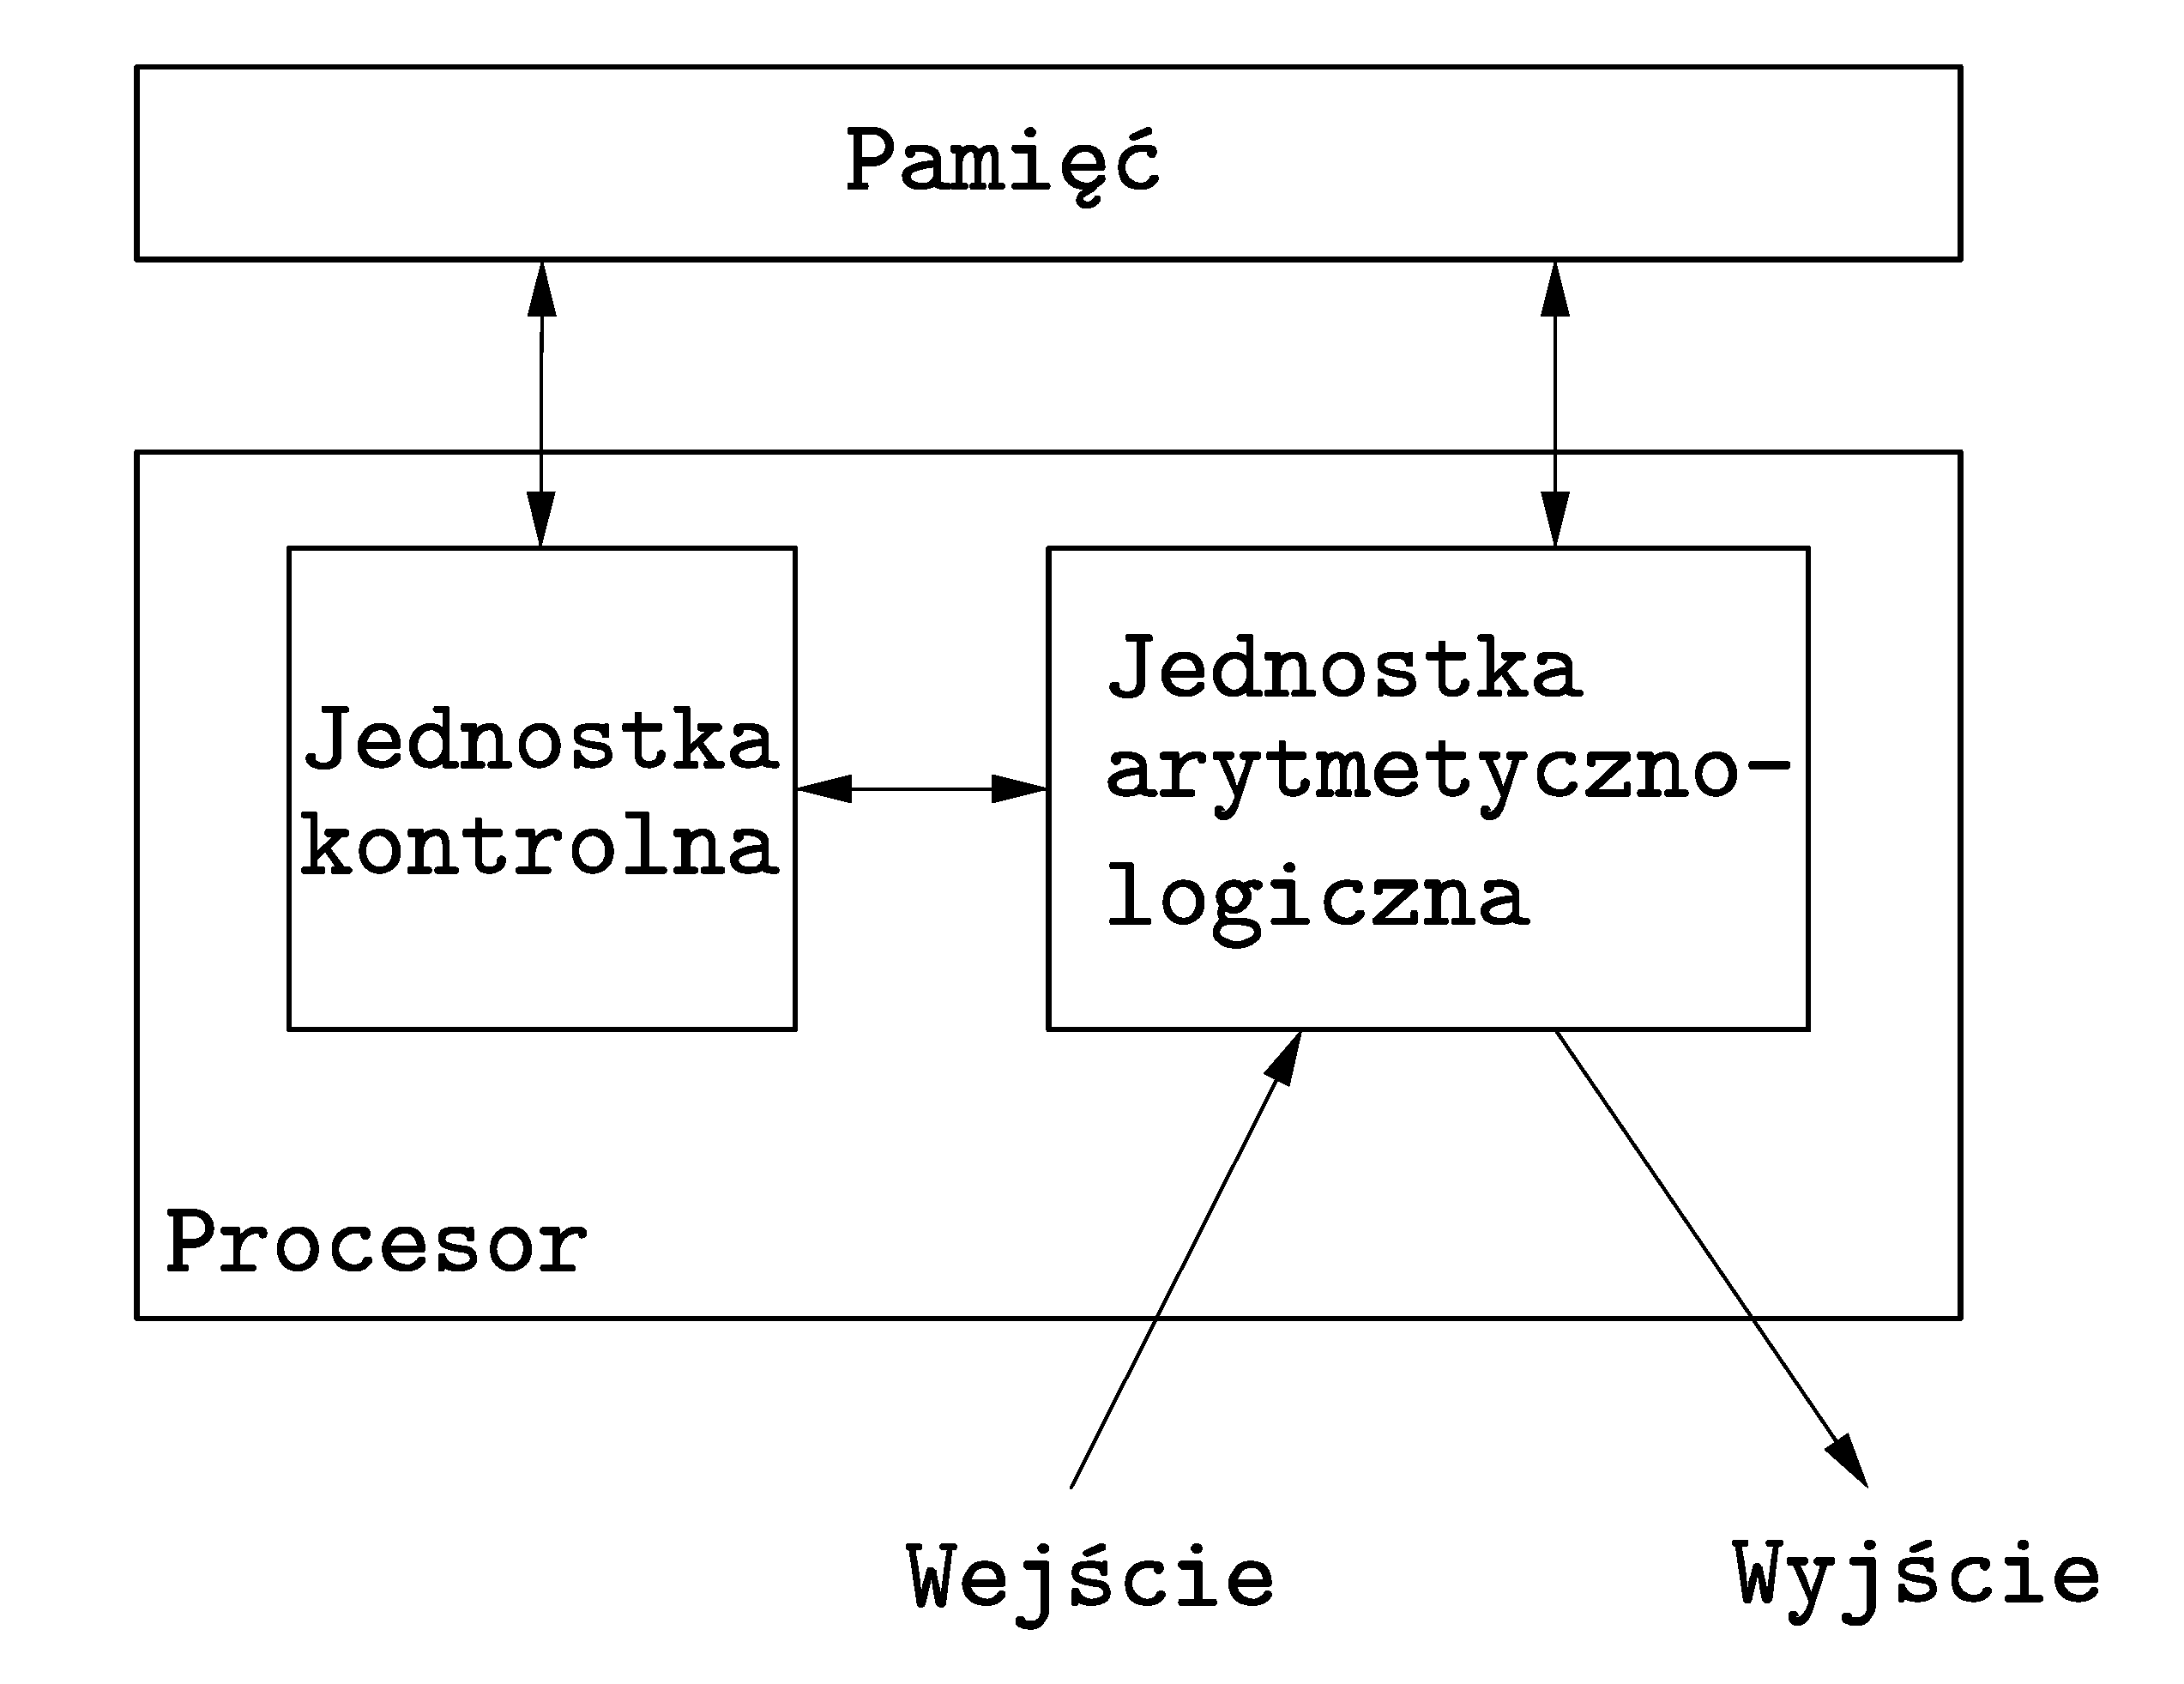
\includegraphics[width=8cm]{images/Rys_Neumann.eps}

\caption{Model obliczeń sekwencyjnych RAM}
\label{fig:neumann}
\end{figure}


% \begin{figure}[h]
% \centering
% 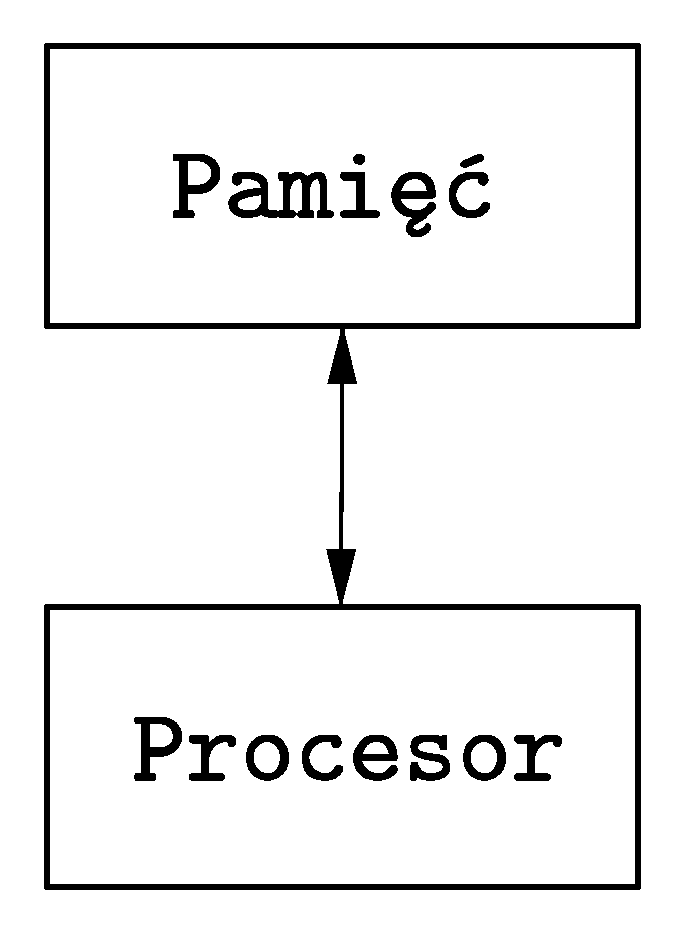
\includegraphics[width=7em]{images/Rys_RAM.eps}
% \caption{Model obliczeń sekwencyjnych RAM}
% \label{fig:ram}
% 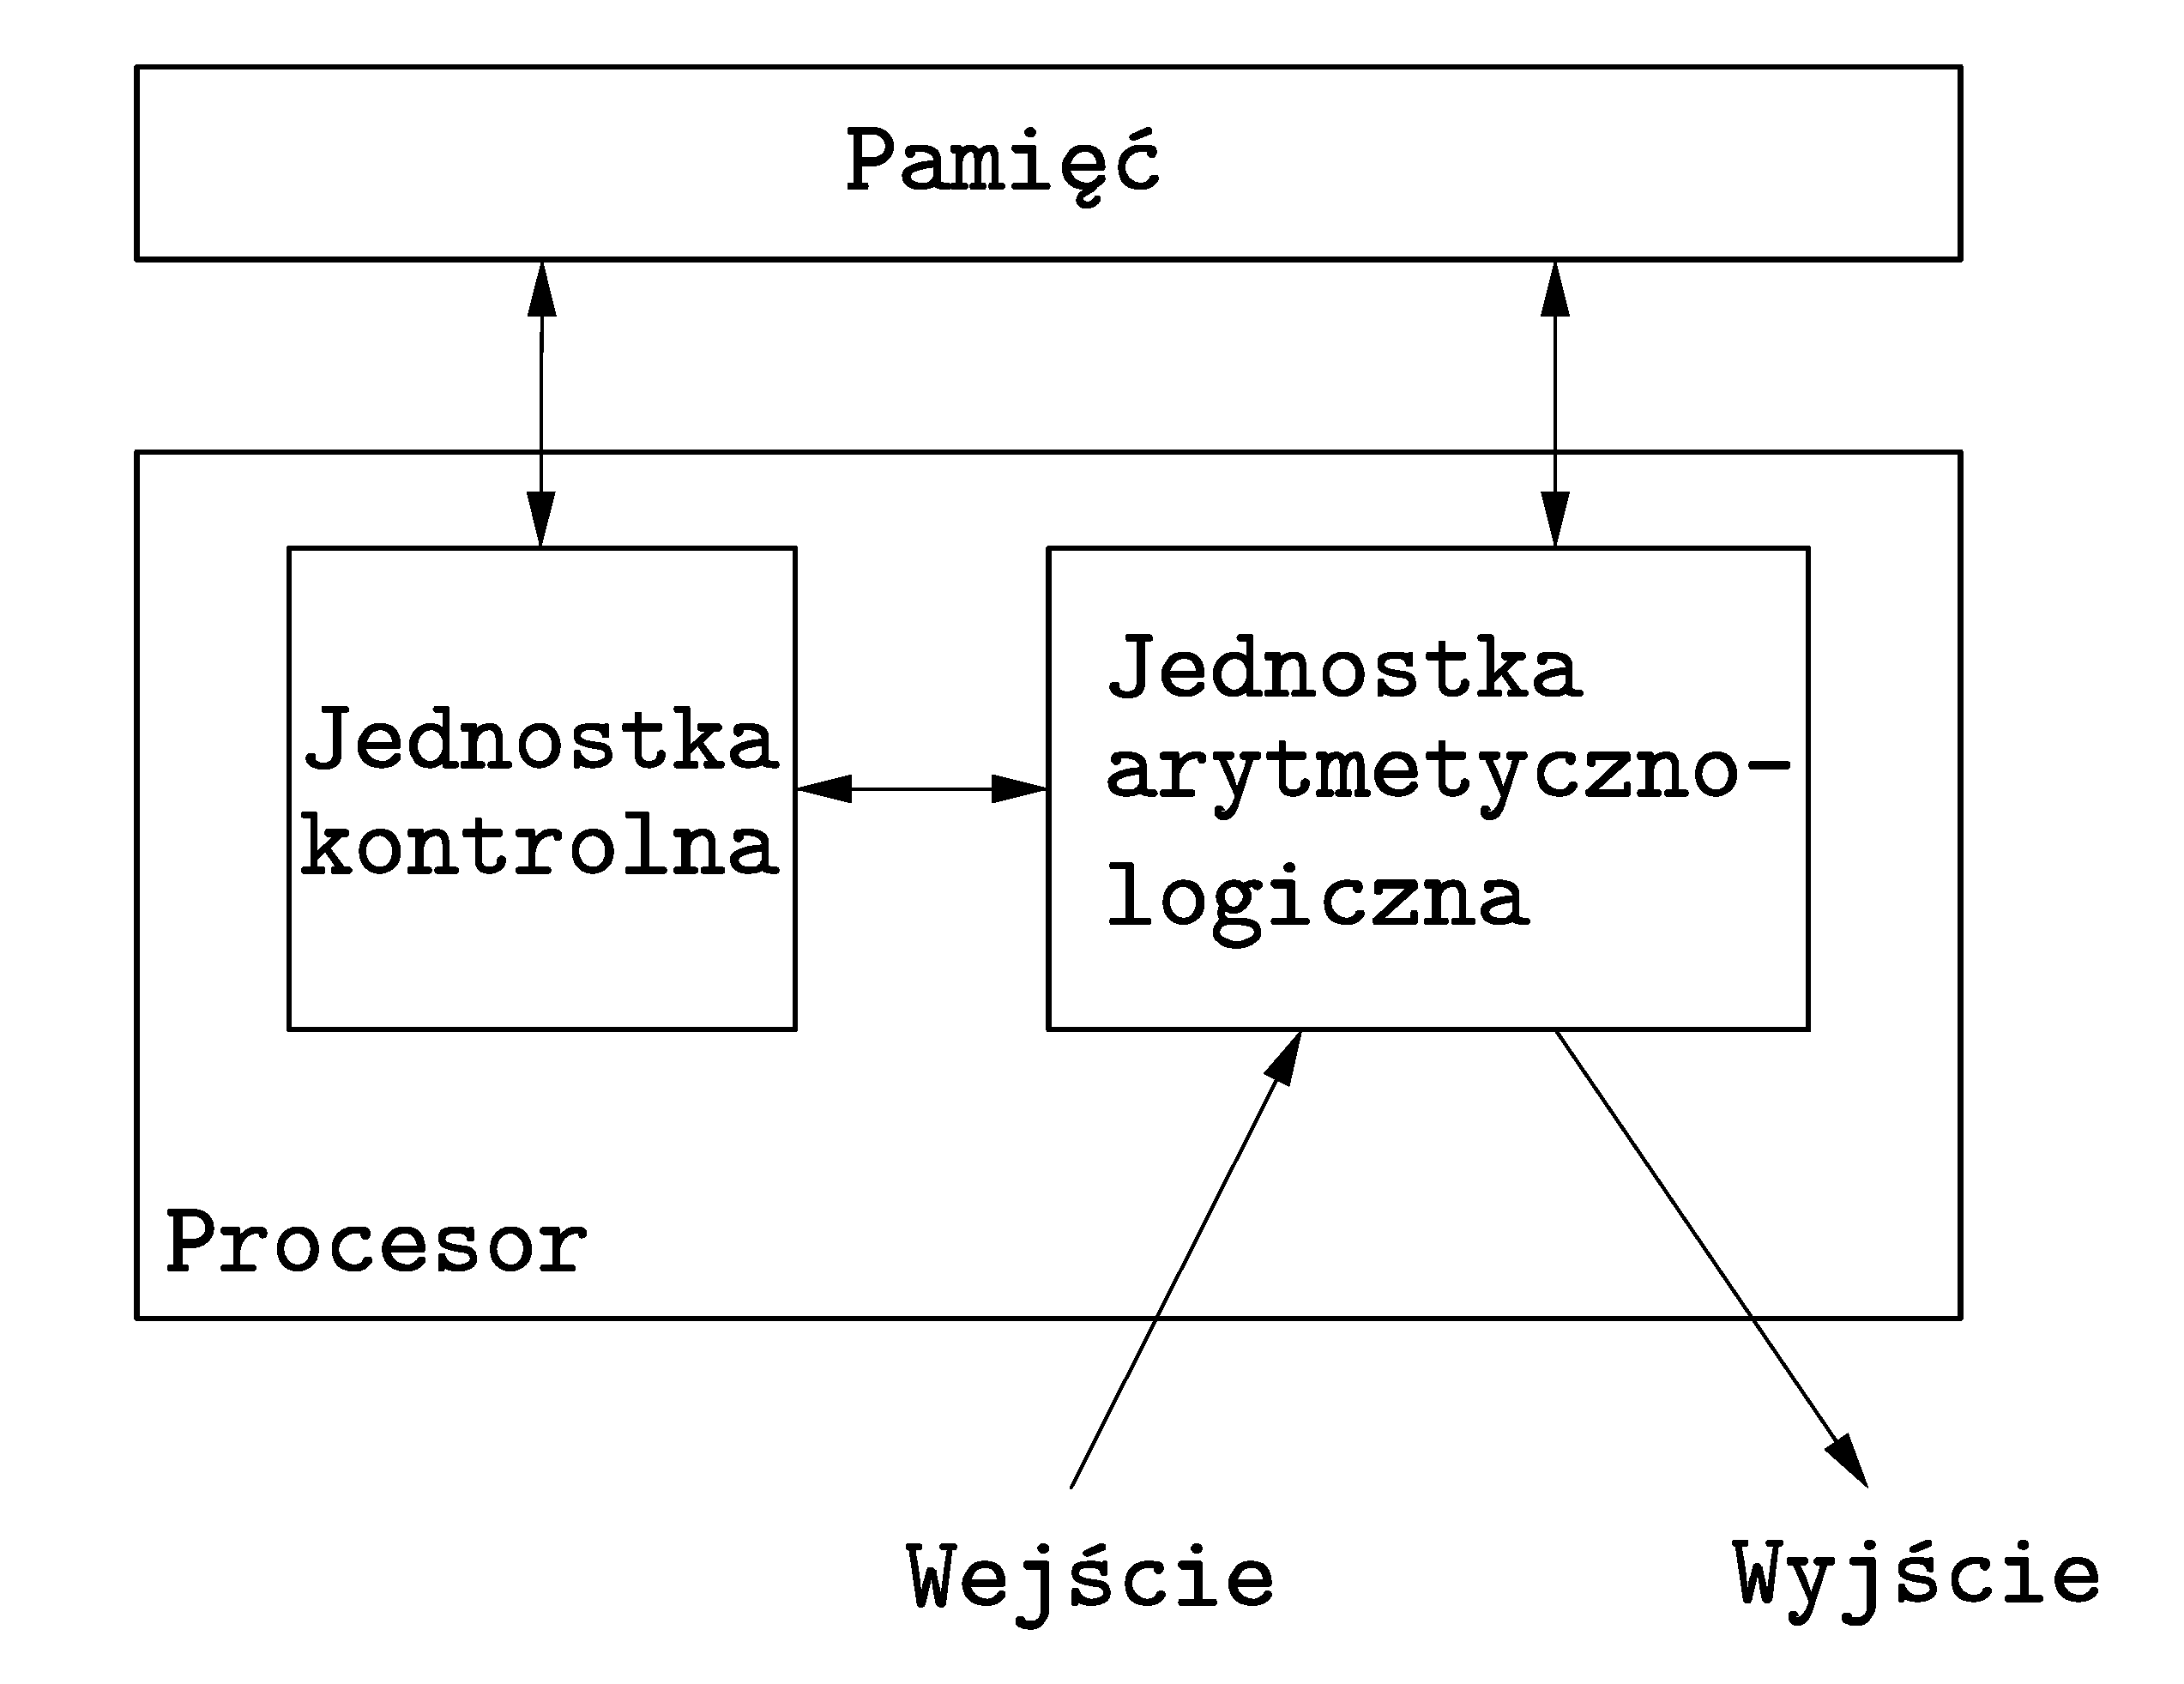
\includegraphics[width=7cm]{images/Rys_Neumann.eps}
% \end{figure}

\begin{table}[H]
\begin{center}
\caption{Przykładowa lista instrukcji procesora\cite{Czech}}
\label{tab:ram_instructions}
\begin{tabular}{|l|c|l|}
\hline
Instrukcja & Argument & Znaczenie \\ \hline
\texttt{LOAD} & \(k, a\) & \(R_k:=w(a)\) \\
\texttt{STORE} & \(k, b\) & \(M_{w(b)}:=R_{k}\) \\
\texttt{ADD} & \(k, c\) & \(R_{k}:=R_{k}+w(c)\) \\
\texttt{SUB} & \(k, c\) & \(R_{k}:=R_{k}-w(c)\)\\
\texttt{MULT} & \(k, c\) & \(R_{k}:=R_{k} \times w(c)\)\\
\texttt{DIV} & \(k, c\) & \(R_{k}:=\lfloor R_{k}/w(c)\rfloor\) \\
\texttt{JUMP} &  \(i\) & \(L:=i\) \\
\texttt{JPOS} & \(k,i\) & \texttt{if} \(R_k>0\) \texttt{then} \(L:=i\) \texttt{else} \(L:=L+1\) \\
\texttt{JZERO} & \(k,i\) & \texttt{if} \(R_k==0\) \texttt{then} \(L:=i\) \texttt{else} \(L:=L+1\) \\
\texttt{JNEG} & \(k,i\) & \texttt{if} \(R_k<0\) \texttt{then} \(L:=i\) \texttt{else} \(L:=L+1\) \\
\texttt{READ} & k & Wczytaj daną z urządzenia zewnętrznego do rejestru \(R_k\) \\
\texttt{WRITE} & k & Wydrukuj daną z rejestru \(R_k\) \\
\texttt{HALT} & & Zakończ obliczenie \\ \hline
\end{tabular}
\end{center}
\end{table}



\label{subsec:PRAM}
\subsection{Model PRAM}

Model wspólnej pamięci składa się z pewnej liczby procesorów, z których każdy posiada własną pamięć i może lokalnie wykonywać programy. Wszystkie procesory mogą komunikować się za pomocą wspólnej globalnej pamięci.\\
Każdemu procesorowi przypożądkowany jest niepowtarzająca się liczba naturalna. Jest to lokalnie dostępny indeks, numer procesora lub jego identyfikator.\\

W modelu wspólnej pamięci wyróżniamy dwa podstawowe tryby operacji. W pierwszym trybie, synchronicznym, wszystkie procesory działają synchronicznie według wspólnego zegara. Model ten nazywamy równoległą maszyną o dostepie swobodnym (PRAM, parallel random-access machine).\\
W drugi trybie, asynchronicznym, każdy procesor pracuje według osobnego zegara. W tym trybie programista jest odpowiedzialny za odpowiednią synchronizację procesorów, jeśli zachodzi taka potrzeba. Dokładniej mówiąc, jeśli procesor ma pobrać dane, to odpowiedzialnością programisty jest upewnienie się, że odpowiednie dane są już uzyskane, ponieważ wartości wspólnych zmiennych są określane dynamicznie w trakcie wykonania programu na różnych procesorach.\\

Ponieważ każdy procesor może uruchomić swój program lokalnie, ten model jest typu MIMD w klasyfikacji Flynna. Znaczy to tyle, że każdy procesor może wykonać pewną instrukcję lub operację na danych niezależnie od tych wykonanych na jakimkolwiek innym procesorze w trakcie danej jednostki czasu.\\

Dla danego algorytmu, rozmiar danych wymienionych pomiędzy pamięcią globalną i pamięcią lokalną różnych procesorów wyraża rozmiar \textbf{komunikacji} wymaganej przez algorytm.



Możemy wyróżnić kilka wariantów modelu PRAM w zależności od wymagań jakie postawimy odnośnie jednoczesnego dostępu kilku procesorów do tego samego adresu w pamięci globalnej.\\
\begin{definicja}{Klasyfikacja PRAM ze względu na dostęp do pamięci}
\begin{itemize}
\item\textbf{EREW} -- algorytmy z wyłącznym odczytem i wyłącznym zapisem; nie pozwala na jednoczesny zapis do pamieci\\
\item\textbf{CREW} -- algorytmy z jednoczesnym odczytem i wyłącznym zapisem; pozwala na jednoczesny  dostęp do pamięci dla instrukcji odczytu\\
\item\textbf{CRCW} -- algorytmy z jednoczesnym odczytem i jednoczesnym zapisem;\\
\item\textbf{ERCW} -- algorytmy z wyłącznym odczytem i jednoczesnym zapisem.\\
\end{itemize}
\end{definicja}

Jeśli nie poczyni się żadnych dodatkowych założeń, to nie jest jasno określone, co zostanie zapisane w komórce pamięci w wyniku jednoczesnego zapisywania do niej przez wiele procesorów w algorytmie typu CRCW. W literaturze można spotkać wiele typów maszyny PRAM, które różnią się sposobami rozwiązywania konfliktów zapisu. Można wśród nich wyróżnić\cite{Cormen94}:

\begin{enumerate}
\item jednolity (ang. common) – procesory muszą zapisać do tej samej komórki pamięci jednolitą wartość
\item dowolny (ang. arbitrary) – zapamiętywana jest dowolna wartość z wartości zapisywanych do tej samej komórki pamięci
\item priorytetowy (ang. priority) – zapamiętywana jest wartość zapisywana przez procesor o najmniejszym numerze
\item (ang. combining) – zapamiętywana jest wartość jest pewną, jednak ściśle określoną kombinacją zapisywanych wartości
\end{enumerate}

\begin{figure}[h]
\centering
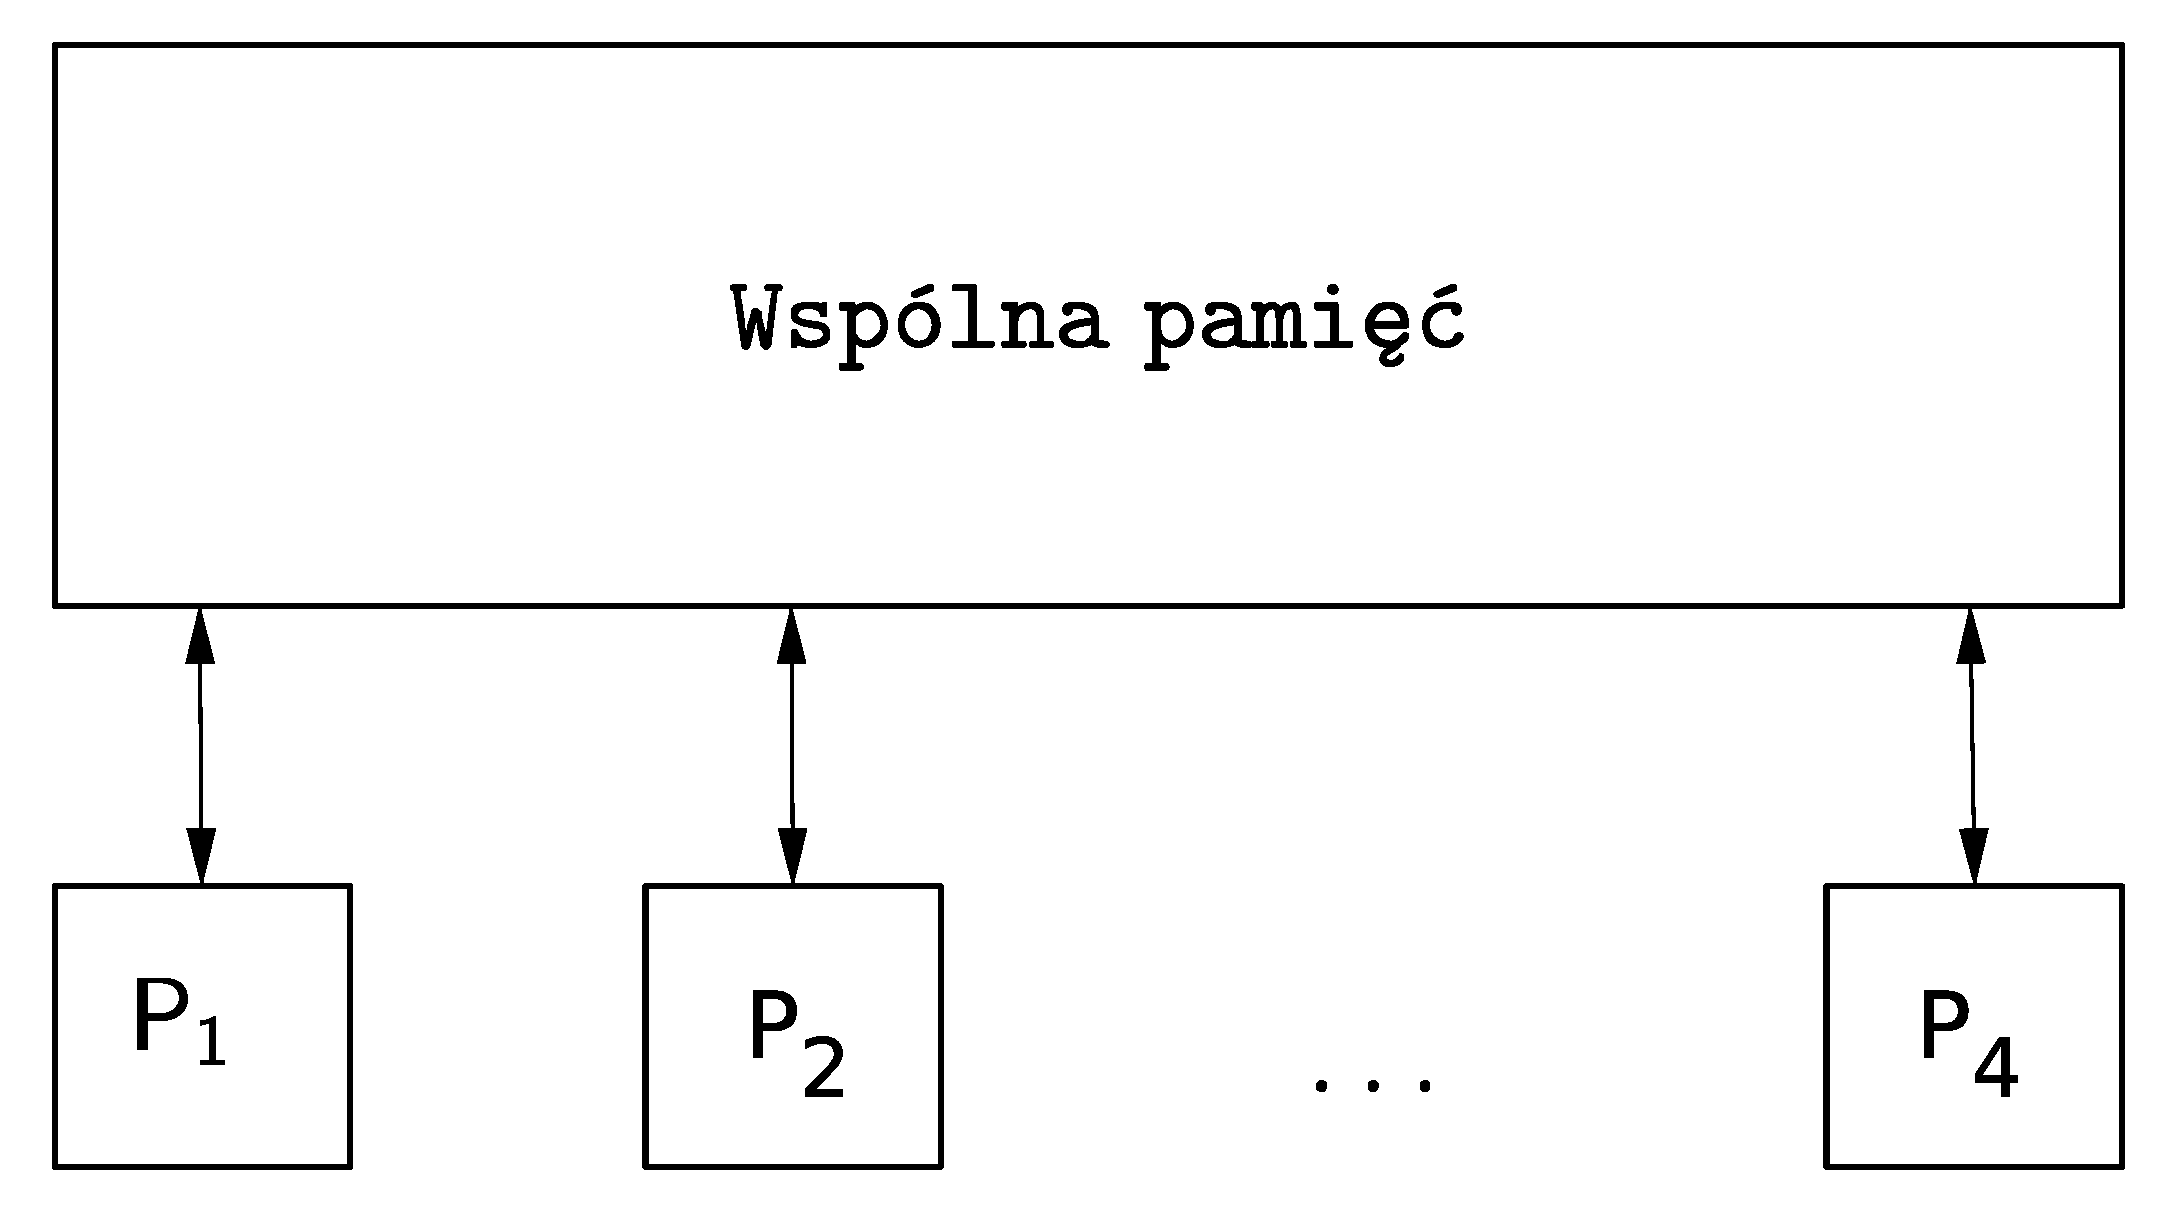
\includegraphics[width=20em]{./images/Rys4.eps}
\caption{Model wspólnej pamięci}
\label{fig:model_shared}
\end{figure}

\subsection{Model sieciowy}

Sieć możemy przedstawić modelowo jako graf \(G=(N,E)\), gdzie każdy węzeł \(i\in N\) oznacza procesor, a każda krawędź \((i, j) \in E\) – dwukierunkową komunikację między procesorami \(i\) i \(j\). Przyjmujemy, że każdy procesor ma swoją lokalną pamięć i nie ma żadnej pamięci współdzielonej przez procesory. Tak jak w przypadku modelu z pamięcią wspólną, operacje w sieci mogą być synchroniczne lub asynchroniczne.\\

W opisie algorytmów dla modelu sieciowego potrzebujemy zdefiniować dwie instrukcje do opisania komunikacji między procesorami.
\begin{enumerate}
 \item send\((X,i)\)
 \item receive\((X,j)\)
\end{enumerate}

Procesor \(P\) wykonujący instrukcję \textbf{send} wysyła kopię \(X\) do procesora \(P_i\), następnie natychmiast przechodzi do wykonywania kolejnej instrukcji.\\
Procesor \(P\) wykonujący instrukcję \textbf{receive} zatrzymuje wykonanie programu aż do chwili, gdy otrzyma dane z procesora \(P_j\), a następnie przechowuje dane w \(Y\) i kontynuuje wykonanie programu.\\



Procesory pracujące w sieci asynchronicznej zarządzają swoimi zadaniami przez wymianę komunikatów. Schemat taki nazywamy modelem wymiany komunikatów. Procesory te niekoniecznie muszą być ze sobą sąsiadujące. 

%\begin{definicja}[Routing]
%Proces dostarczania każdego komunikatu od źródła do przeznaczenia nazywmy routingiem.
%\end{definicja}

Charakterysuje ją kilka parametrów:

\begin{enumerate}
 \item średnica – maksymalna odległość (krawędziowa) między dowolną parą węzłów; im miejsza, tym lepiej.
 \item maksymalny stopień wierzchołka – maksymalna liczba łączy do dane procesora
 \item szerokość połowienia sieci – minimalna liczba krawędzi, które muszą zostać usunięty, aby podzielić ją na dwie równe podsieci
 \item spójność krawędziowa – minimalna liczba krawędzi, które muszą ulec awarii, aby sieć stała się niespójna
 \item koszt sieci – koszt wykonania, zarządzania i utrzymania połączeń między procesorami; w najprostrzym przypadku mierzony liczbą krawędzi
\end{enumerate}


\subsubsection{Sieć liniowa}
\begin{definicja}[Sieć liniowa]
Model składa się z \(p\) procesorów \(P_1, P_2, \dots, P_p\) połączonych ze sobą w ciąg, tzn. procesor \(P_i\) połączony jest z procesorem \(P_{i-1}\) i \(P_{i+1}\), o ile takie istnieją. Średnica takiej sieci wynosi \(p-1\), jej maksymalny stopień wynosi \(2\).\\
\end{definicja}
\begin{definicja}[Torus]
Sieć liniowa z połączonymi końcami.
\end{definicja}


\subsubsection{Sieć dwuwymiarowa}

Dwuwymiarowa sieć jest dwuwymiarową wersją sieci liniowej. Składa się ona z \(p=m^2\) procesorów ułożonych w siatkę \(m\times m\) taką, że procesor \(P_{i,j}\) jest połączony z procesorem \(P_{i\pm 1, j}\) i \(P_{i, j\pm 1}\).\\
Średnica takiej sieci złożonej z \(p=m^2\) procesorów wynos \(\sqrt{p}\) a jej maksymalny stopień \(4\)


\subsubsection{Sieć hipersześcienna}

\begin{definicja}{Kostka Boola}\\
Niech \(i_{d-1}i_{d-2}\dots i_{0}\), gdzie \(0\leq i \leq p-1\) będzie binarną reprezentacją \(i\). Wówczas procesor \({i}\) jest połaczony z procesorem \(P_{i^(j)}\), gdzie \(i^{(j)}=i_{d-1}\dots \overline{i_j} \dots i_0\) i \(\overline{i_j} = 1 - i_j\). Innymi słowy, dwa procesory są ze sobą połączone wtedy i tylko wtedy, gdy ich wskaźniki różnią się tylko jednym bitem.\\
\end{definicja}

Sieć w topologii hipersześcianu skłąda się z \(p=2^d\) procesorów połączonych w d-wymiarową kostkę Boola.\\

Hipersześcian ma strukurę rekursywną. Kostkę \(d\)-wymiarową możemy rozszerzyć do \(d+1\) wymiarów przez połączenie poszczególnych procesorów do \(d\)-wymiarowych kostek.\\

Średnica d-wymiarowego hipersześcianu wynosi \(d=\log{p}\). Jest tak ponieważ odległośc w grafie między dwoma procesorami \(P_i\) i \(P_j\) jest równa liczbie pozycji bitów, którymi wskaźniki \(i\) i \(j\) różnią się między sobą. Stąd jest ona mniejsza lub równa \(d\), a ponadto odległość między \(P_0\) a \(P_{2^d-1}\) wynosi d. Każdy węzeł jest stopnia \(d=\log{p}\).

\begin{figure}[h]
\centering
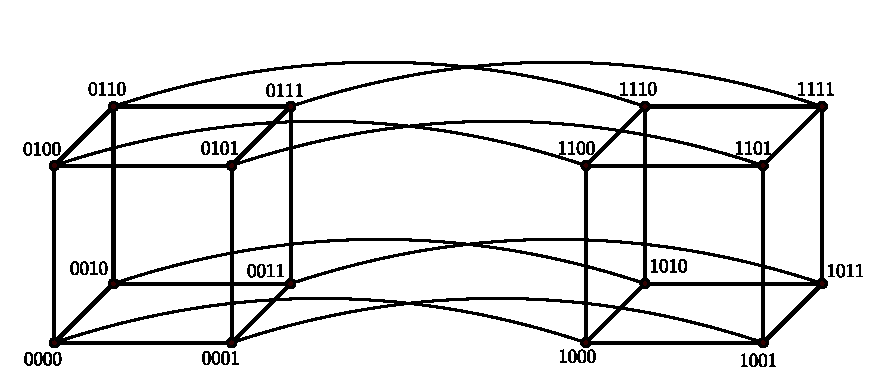
\includegraphics[width=36em]{./images/systolic.eps}
\caption{Sieć w topologii hipersześcianu}
\label{fig:systolic}
\end{figure}